\clearpage
\section{Implementation}

4 Implementation
[You may structure this as you wish, but make the description complete, including choices of
technology e.g. tools, libraries and relevant configuration. This should include evaluation.]





-----------------------------------------------------------
--moove to th eimplementation

\paragraph{Selected Features and Removed Features}
Based on our correlation analysis (based on the Figure~\ref{fig:app-correlation}), the 
following feature selection decisions were made (Table~\ref{tab:feature_selection}):

\begin{table}[H]
    \centering
    \caption{Feature Selection Based on Correlation Analysis}
    \label{tab:feature_selection}
    \begin{tabular}{cccc}
        \hline
        \textbf{Category} & \textbf{Kept Features} & \textbf{Removed Features} & \textbf{Reason} \\
        \hline\hline
        \textbf{Price} & Close & Open, High, Low & Highly correlated \\
        \textbf{Trend} & \acrshort{sma} & \acrshort{ema}, \acrshort{wma} & Highly correlated \\
        \textbf{Momentum} & \acrshort{macd} Histogram & \acrshort{macd} Signal & Derivative of MACD \\
        \textbf{Volatility} & \acrshort{bb} (Middle) & \acrshort{bb} (Lower / Upper) & Derived \\
        \textbf{Oscillators} & \acrshort{sso} D & \acrshort{sso} K & Redundant \\
        \hline
    \end{tabular}
\end{table}

\begin{figure}[H]%
    \centering
    \caption{Correlation Matrix For the Workday's Stock Dataset}
    \label{fig:app-correlation}
    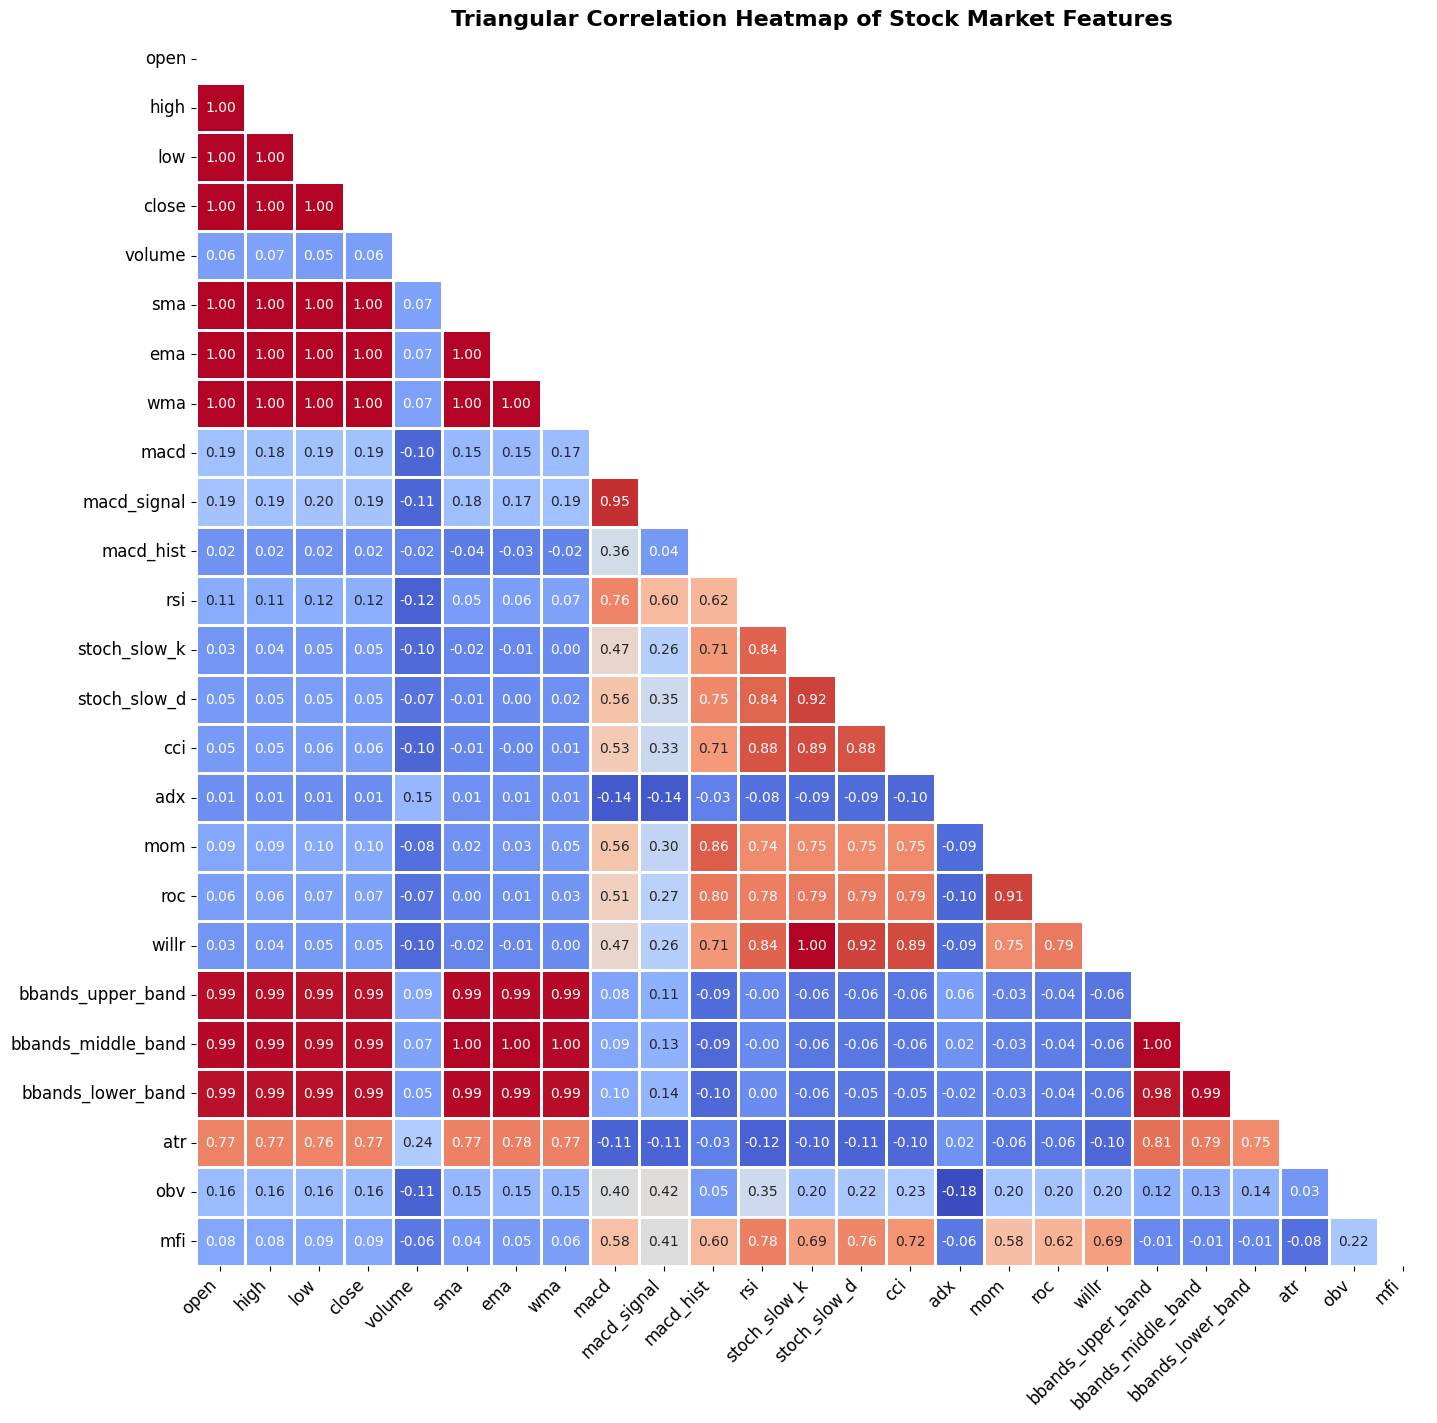
\includegraphics[width=\linewidth]{img/sections/main/correlation.png}
\end{figure}

By applying this feature selection process, we ensure that the dataset remains informative 
while avoiding unnecessary complexity. This streamlined feature set enhances model
generalization, improves training efficiency, and mitigates the risk of 
overfitting~\parencite{shaban2024SMPDL, phuoc2024StockPrediction}.

\paragraph{Summary of Feature Selection} The selected features presented in the
Table~\ref{tab:feature_selection_kept} provide 
\emph{unique information without excessive correlation}.

\begin{table}[H]
    \centering
    \caption{Feature Selected}
    \label{tab:feature_selection_kept}
    \begin{tabular}{ccp{8cm}}
        \hline
        \textbf{Category} & \textbf{Feature} & \textbf{Justification} \\
        \hline\hline
        Target & Close Price & Target variable for stock prediction. \\
        Volume & Volume & Measures market activity and confirms trends. \\
        Trend  & \acrshort{sma} & Tracks long-term price trends.\\
        Momentum & \acrshort{macd} Histogram & Captures momentum. \\
        Volatility & \acrshort{bb} Middle & Represents volatility without 
        redundant Upper/Lower bands. \\
        Oscillators & \acrshort{sso} D & More stable than Slow K, useful for 
        overbought/oversold conditions. \\
        Trend & \acrshort{adx} & Measures trend strength but not direction. \\
        Momentum & \acrshort{rsi} & Identifies potential price reversals
        using price momentum. \\
        Volatility & \acrshort{atr} & Measures price fluctuation and risk. \\
        Volume & \acrshort{obv} & Confirms price movements using volume 
        trends. \\
        Volume & \acrshort{mfi} & Combines price and volume to detect
        overbought/oversold conditions. \\
        \hline
    \end{tabular}
\end{table}

Since the dataset contains a manageable number of features (~20-25),
dimensionality reduction techniques such as \acrfull{pca}
are not required. 

The target variable in this dataset is the Close Price, representing the final
traded price of a stock at the end of each trading period, which serves as the
primary dependent variable for forecasting future stock movements.


\subsubsection{Hyperparameters selection}

\paragraph{Number of Neurons and Layers} The choice of hidden layers and the number of neurons per 
layer significantly impacts the model’s capacity and ability to generalize. Based on empirical 
studies~\parencite{chang2024StockPrediction, nabipour2020DeepLearning}, 
the following guidelines are recommended:

\begin{table}[H]
\centering
\caption{Recommended Neurons and Layers for LSTM Variants}
\label{table:neurons_layers}
\begin{tabular}{cccp{5cm}}
\hline
\textbf{Model Type} & \textbf{Hidden Layers} & \textbf{Neurons per Layer} & \textbf{Use Case} \\ \hline\hline
LSTM & 1-3 & 50-200 & Basic time-series forecasting \\
LSTM-GRU & 2-4 & 100-300 & Hybrid efficiency for sequence learning \\
LSTM-BiGRU & 3-5 & 150-400 & Bidirectional dependency capture \\
\hline
\end{tabular}
\end{table}

\paragraph{Hyperparameter Tuning}
Key hyperparameters and their recommended values are shown in Table~\ref{table:hyperparams}.

\begin{table}[H]
\centering
\caption{Hyperparameter Recommendations for LSTM Models}
\label{table:hyperparams}
\begin{tabular}{ccp{6.5cm}}
\hline
\textbf{Hyperparameter} & \textbf{Recommended Range} & \textbf{Description} \\ \hline\hline
Learning Rate & 0.001 - 0.0001 & Controls step size during optimization~\parencite{parmar2018stock} \\
Batch Size & 32-128 & Affects training stability and convergence \\
Optimizer & Adam, RMSprop & Commonly used for recurrent networks \\
Dropout Rate & 0.2 - 0.5 & Prevents overfitting~\parencite{agrawal2022StockPrediction} \\
Number of Epochs & 50 - 200 & Determines training iterations \\
Activation Function & Tanh, ReLU & Tanh preferred for LSTMs \\
Batch Normalization & Applied & Stabilizes training and accelerates 
convergence~\parencite{balasubramanian2023SystematicSurvey} \\
Early Stopping & Used & Prevents unnecessary computation by halting when validation loss 
stops improving~\parencite{chang2024StockPrediction} \\
\hline
\end{tabular}
\end{table}

\paragraph{Forget Gate Tuning and Avoiding Vanishing Gradients}
The forget gate in LSTM-based models regulates how much past information is discarded. Setting the 
forget bias close to 1 (e.g., $ b_f = 1 $) ensures longer 
retention~\parencite{balasubramanian2023SystematicSurvey}. Additionally, gradient 
clipping (e.g., max norm of 5) and layer normalization help prevent exploding and vanishing 
gradients~\parencite{chang2024StockPrediction}.

\paragraph{Optimal Lookback Period for Time-Series Forecasting} Selecting an appropriate number
of past days for prediction significantly affects model accuracy. General 
recommendations~\parencite{shaban2024SMPDL, phuoc2024StockPrediction} are shown in Table~\ref{table:lookback}.

\begin{table}[H]
\centering
\caption{Recommended Lookback Days for LSTM Models}
\label{table:lookback}
\begin{tabular}{cc}
\hline
\textbf{Prediction Horizon} & \textbf{Recommended Lookback Days} \\ \hline\hline
Short-term (1-5 days ahead) & 30-60 days \\
Medium-term (5-30 days ahead) & 90-180 days \\
Long-term (30+ days ahead) & 180-365 days \\\hline
\end{tabular}
\end{table}











